\chapter{Evaluation}

Um es zu überprüfen, ob die Ziele dieses Projektes erreichtet werden, wird eine Studie durchgeführt. In diesem Kapitel geht es um den Entwurf der Studie und die gesammelten Daten durch die Studie.

\section{Entwurf der Studie}

Die Hauptziele der Studie sind, der Lerneffekt der VR Übung und die Benutzererfahrung der WebVR Applikation zu beurteilen. Die Studie wird um die Ziele entworfen.

\subsection{Entwurf der Test und Fragebogen}

Das Projekt wird von zwei Aspekten austestet. Der Lerneffekt der VR Übung und die Benutzererfahrung der VR Applikation. Deswegen werden die Teile der Studie für jeden Aspekt getrennt entworfen.

\subsubsection{Lerneffekt durch die VR Übung}

Da die VR Übung wird in dem Learning Management System Moodle integriert wird, kann der Lerneffekt durch der Test Aktivität überprüft wird. Fünf Aufgaben werden in der Test Aktivität eingefügt, damit von der Reihenfolge der Infusinosvorbereitung bis kleine Forderung eines Abschnitts überprüft werden.

\begin{enumerate}
    \item \textbf{Reihenfolge ordnen}
    
    Die achten Abschnitte der Infusionsvorbereitung werden ungeordnet dargestellt. Sie sollen nach der richtigen Reihenfolge geordnet werden. Durch diese Aufgabe wird es prüft, ob der Lernende dem Ablauf einer Infusionsvorbereitung eingeprägt ist. (Abbildung ~\ref{fig:Aufgabe1})
    
\begin{figure}[ht]
\vspace*{1em}
\centering
\caption{Aufgabe: Reihenfolge}
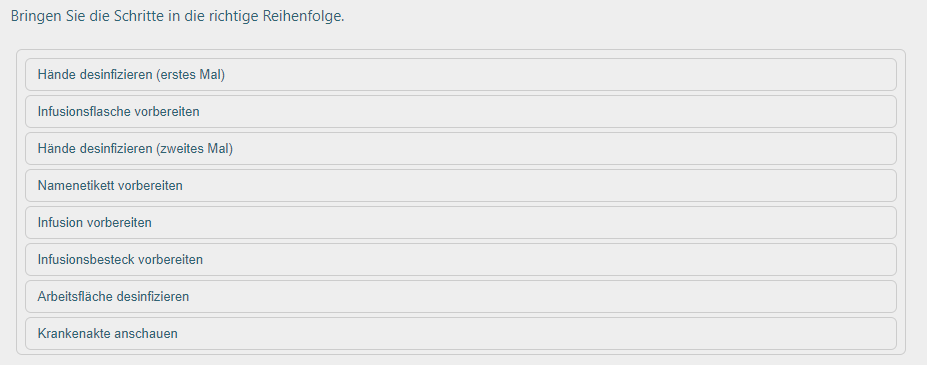
\includegraphics[width=\textwidth]{images/Aufgabe1.png}
\label{fig:Aufgabe1} 
\end{figure}
    
    
    \item \textbf{5R auswählen}
    
    5R sind die wichtigen Informationen auf der Krankenakte, die während der Vorbereitung zuerst gecheckt werden sollen. Fünf richtige Optionen sollen von 8 Optionen ausgewählt. Durch diese Aufgabe wird es prüft, ob der Lernende gelernt hat, was die wichtigen Informationen für die Infusionsvorbereitung sind. (Abbildung ~\ref{fig:Aufgabe2})
    
\begin{figure}[ht]
\vspace*{1em}
\centering
\caption{Aufgabe: 5R-Regel}
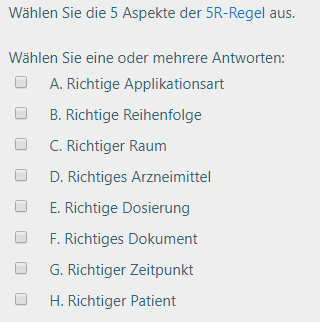
\includegraphics[width= 0.5\textwidth]{images/Aufgabe2.png}
\label{fig:Aufgabe2} 
\end{figure}
    
    \item \textbf{Status der Rollenkleme}
    
    Während der Infusionsvorbereitung ist es wichtig, die Rollenkleme auf den entsprechenden Zeitpunkten zu öffnen und schließen. Durch die Aufgabe wird es überprüft, ob der Lernende die richtigen Zeitpunkte gemerkt. (Abbildung ~\ref{fig:Aufgabe3})
    
\begin{figure}[ht]
\vspace*{1em}
\centering
\caption{Aufgabe: Rollenklemme}

\includegraphics[width= \textwidth]{images/Aufgabe3.png}
\label{fig:Aufgabe3} 
\end{figure}
    
    \item \textbf{Handschuhe tragen}
    
    Sicherheit ist ein wichtiges Thema. Durch Handschuhe werden die Hände geschützt. Bei dieser Aufgabe werden achte Abschnitte aufgelistet, und einer davon ausgewählt werden soll, während deren Handlung Handschuhe eingetragen werden. Durch diese Aufgabe wird das Sicherheitsbewusstsein des Lernenden überprüft. (Abbildung ~\ref{fig:Aufgabe4})
    
\begin{figure}[ht]
\vspace*{1em}
\centering
\caption{Aufgabe: Handschuhe}
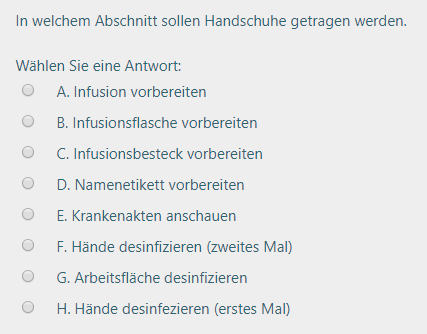
\includegraphics[width= 0.5\textwidth]{images/Aufgabe4.png}
\label{fig:Aufgabe4} 
\end{figure}
    
    \item \textbf{Infusionsflasche prüfen}
    
    Um die Benutzbarkeit der Infusionsflasche zu bestimmen, soll die Infusionsflasche vor der Nutzung gecheckt werden, nämlich die Kappe, die Flüssigkeit und das Etikett. Vier Optionen werden aufgelistet, und die drei richtigen Optionen sollen ausgewählt werden. Durch diese Aufgabe wird es überprüft, ob der Lernende das Bewusstsein hat, die Benutzbarkeit der Materialien zu checken. (Abbildung ~\ref{fig:Aufgabe5})
    
\begin{figure}[ht]
\vspace*{1em}
\centering
\caption{Aufgabe: Handschuhe}
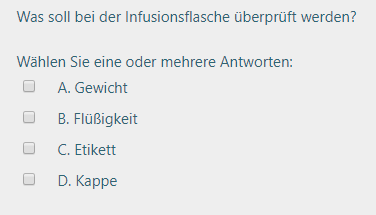
\includegraphics[width= 0.5\textwidth]{images/Aufgabe5.png}
\label{fig:Aufgabe5} 
\end{figure}
    
\end{enumerate}

\subsubsection{Benutzererfahrung der VR Applikation}

Die Benutzererfahrung ist ziemlich subjektiv, deswegen wird ein Fragebogen erstellt, um die Feedbacks der Benutzer zu sammeln.

Um die Benutzererfahrung umfassend zu berichten, wird der Fragebogen nach den sechs Kategorien \citep{28} entworfen. Da die Benutzererfahrung zusammengefasst ist, ist es schwierig, nach jeder einzigen Kategorie Frage zu stellen. Deswegen können die Fragen auch mehrere Kategorien betreffen.

Jede Frage beseht aus zwei Teile. Einer davon ist eine pflichte Frage im Form Ratingskalen. Der andere ist eine entsprechende optionale Frage im Form Meinungsfrage.

\begin{enumerate}
    \item Ich habe das Gefühl, wirklich eine Infusion vorzubereiten.
    
    Wenn nein, was ist die Ursache (z.B. Mangel der Geräusche)?
    
    (Extensiveness, Matching, Surroundness, Vividness, Interactability)
    
    \item Während der Übung weiß ich, was und wie ich tun soll.
    
    Wenn nein, was ist unklar?
    
    (Interactability, Plot)
    
    \item Ich kann das Zielobjekt mühelos finden.
    
    Wenn nein, was ist nicht einfach zu finden?
    
    (Matching, Surroundness, Vividness)
    
    \item Ich bin immer sicher, dass jede Aktion von mir auf den Objekten durchgeführt wird. Wenn das Objekt nicht reagiert, kann mit dem Objekt auch nicht interagiert werden.
    
    Wenn nein, was funktioniert nicht?
    
    (Interactability, Plot)
    
    \item  Die Feedbacks der Objekte nach der Interaktion habe ich erwartet. 
    
    Wenn nein, was ist unerwartet?
    
    (Matching, Interactability)
    
    \item Ich kann die wichtige Informationen (z.B. 5R, Etiketten) deutlich sehen.
    
    Wenn nein, was ist undeutlich?
    
    (Surroundness, Vividness)
    
\end{enumerate}

Whiteboard wird als Hilfsmittel entworfen. Um der Effekt des Whiteboards zu untersuchen, werden die Fragen über der Nutzung von Whiteboard in den Formen Entscheidungsfragen und Ratingskalen gestellt.

\begin{enumerate}
    \item Ich habe die Hinweise auf dem Whiteboard benutzt.
    
    Wenn ja, sind die Hinweise hilfreich?
\end{enumerate}

Für das ganze Projekt werden die Fragen über der Integration zwischen LMS und die WebVR Applikation in den Formen Ratingskalen und Meinungsfrage und die Frage über dem Lerneffekt im Form Ratingskalen gestellt.

\begin{enumerate}
    \item Ich glaube, dass die VR Übung gut in den Unterricht integriert ist.
    
    Wenn nein, was gefällt Ihnen nicht?
    
    \item Wie gut ist der Lerneffeket im Vergleich mit der realen Praxis? 
\end{enumerate}

Am Ende des Fragebogens werden zwei allgemeine Meinungsfragen gestellt, um die Gedanken der Versuchspersonen zu sammeln.

\begin{enumerate}
    \item Was gefällt Ihnen während der Übung?
    
    \item Was gefällt Ihnen während der Übung nicht?
\end{enumerate}

\subsection{Entscheidung der Geräten}

Da WebVR cross-plattform ist, wird die Studie mit unterschiedlichen Geräten gemacht. Allerdings ist es wegen der Begrenzung der Zeit und des Mangels an Versuchsperson nicht möglich, mit alle verfügbare Geräten Studie zu machen, deswegen werden drei Geräte entschieden.

\begin{itemize}
    \item \textbf{PC}: beste Erreichbarkeit
    \item \textbf{Smartphone}: beste Mobilität
    \item \textbf{HTC Vive}: bestes VR Erlebnis
\end{itemize}

\subsection{Entwurf des Ablaufs}

Insgesamt 15 Versuchspersonen nehmen die Studie teil. Sie sind kein Pfleg-Studenten und haben keine Vorwissen über Infusionsvorbereitung, damit können die Lerneffekte des Unterrichts und der VR Übung berichtet werden.

Jede Gerät wird von fünf Versuchspersonen benutzt. Jede Versuchsperson soll die Untersuchung allein machen.

Die Versuchsperson wird gefordert, zuerst mit den Materialien (Text, Video und Diagramm) zu lernen, und den Test machen. Das Ergebnis der Tests wird nicht der Versuchsperson informiert, sondern als Controllergruppe gespeichert.

Danach soll die Versuchsperson die VR Übung machen und den Test noch einmal machen. Die Zwei Ergebnisse werden mit einander vergleicht, um der Effekt der Übung zu finden.

Am Ende der Studie soll die Versuchsperson einen Fragebogen erfüllen, um die Benutzererfahrung der WebVR Applikation zu beurteilen.

\section{Daten der Studie}

\section{Diskussion}

\subsection{Probleme}
\begin{itemize}
    \item \textbf{Objekte schwer zu finden (Smartphone > PC > Vive)}
    
    Das Problem erscheint auf alles drei Geräten. Das Problem auf Smartphone und PC ist schlimmer als auf HTC Vive. Es gibt zwei Gründe für die Schwierigkeit, die Objekte zu finden.
    
    Der erste Grund ist, dass die Umgebung und die Objekte für die Versuchspersonen, die kein Pflege-Studenten sind, fremd sind. Es passierte mehrere Mal, dass die Versuchspersonen nicht wissen, wo die Krankenakte und die Einmalhandschuhe gelegt werden, weil die Krankenakte geschlossen ist und der Spender für Einmalhandschuhe nicht bekannt ist.
    
    Der zweite Grund ist, dass die Ansicht von PC und Smartphone klein ist. Die Hängeschränke sind sogar nicht in der Sicht des Smartphones nach der Initialisierung.
    
    Um das Problem zu lösen, sollen die Umgebung und die Objekte in dem Unterricht als Vorwissen vorgestellt werden, oder soll eine Leitung über der Umgebung und den Objekten in der VR Umgebung vor dem Start der Übung geboten.
  
    \item \textbf{Fehlen des aktiven Hinweises}
    
    In der VR Umgebung wird die Hinweise durch dem Whiteboard dargestellt. Allerdings ist es ein passive Angebot. Das heißt, dass die Hinweise ignoriert werden, wenn der Benutzer nicht an dem Whiteboard schaut. Deswegen passiert es, dass die Versuchsperson lange Zeit auf den falschen Objekten konzentriert, weil er nicht rechtzeitig an dem Whiteboard schauet.
    
    Um das Problem zu lösen, soll ein aktiver Hinweis eingesetzt werden, d.h. direkt vor den Augen zum richtigen Zeitraum darzustellen. Der Hinweis kann ein Vorschlag sein, dem Whiteboard anzuschauen.
    
    \item \textbf{Die Entfernung der Einmalhandschuhe nicht deutlich}
    
    Nach der Desinfektion der Arbeitsfläche werden die Merkmale der Einmalhandschuhe (Einmalhandschuhe Modell vor der Augen in PC und Smartphone und blauer Farbe auf der Hände in Vive) entgefernt. Aber die Entfernung ist nicht deutlich, weil es keine Animation dafür gibt. Sodass merken manche Versuchspersonen nicht, wann die Handschuhe entfernt werden.
    
    Mit einer Animation für die Entfernung kann das Problem behoben werden.
    
    
    
    \item Lokation Veränderung nicht einfach (PC)
    Geschwindigkeit zu schnell
    \item VR Geräte zu benutzen
    Die Versuchspersionen sind wegen der Mangel der VR Erfahrung nicht an den VR Geräten und den Controllers gewohnt
\end{itemize}

\subsection{Vorteile}
\begin{itemize}
    \item Guter Lerneffekt
    \item Immersive Erfahrung
    \item Gute Leitung auf dem Whiteboard
    \item Geräusch Feedbacks
    \item gute integriert mit LMS
    
\end{itemize}











